\chapter{Inheritance}

In this chapter I present classes to represent playing cards,
decks of cards, and poker hands.  If you don't play poker, you can
read about it at \url{http://en.wikipedia.org/wiki/Poker}, but you don't have
to; I'll tell you what you need to know for the exercises.
Code examples from this chapter are available from
\url{http://thinkpython.com/code/Card.py}.
\index{playing card, Anglo-American}
\index{card, playing}
\index{poker}

If you are not familiar with Anglo-American playing cards,
you can read about them at \url{http://en.wikipedia.org/wiki/Playing_cards}.


\section{Card objects}

There are fifty-two cards in a deck, each of which belongs to one of
four suits and one of thirteen ranks.  The suits are Spades, Hearts,
Diamonds, and Clubs (in descending order in bridge).  The ranks are
Ace, 2, 3, 4, 5, 6, 7, 8, 9, 10, Jack, Queen, and King.  Depending on
the game that you are playing, an Ace may be higher than King
or lower than 2.
\index{rank}
\index{suit}

If we want to define a new object to represent a playing card, it is
obvious what the attributes should be: {\tt rank} and
{\tt suit}.  It is not as obvious what type the attributes
should be.  One possibility is to use strings containing words like
\verb"'Spade'" for suits and \verb"'Queen'" for ranks.  One problem with
this implementation is that it would not be easy to compare cards to
see which had a higher rank or suit.
\index{encode}
\index{encrypt}
\index{map to}
\index{representation}

An alternative is to use integers to {\bf encode} the ranks and suits.
In this context, ``encode'' means that we are going to define a mapping
between numbers and suits, or between numbers and ranks.  This
kind of encoding is not meant to be a secret (that
would be ``encryption'').

\newcommand{\mymapsto}{$\mapsto$}

For example, this table shows the suits and the corresponding integer
codes:

\begin{tabular}{l c l}
Spades & \mymapsto & 3 \\
Hearts & \mymapsto & 2 \\
Diamonds & \mymapsto & 1 \\
Clubs & \mymapsto & 0
\end{tabular}

This code makes it easy to compare cards; because higher suits map to
higher numbers, we can compare suits by comparing their codes.

The mapping for ranks is fairly obvious; each of the numerical ranks
maps to the corresponding integer, and for face cards:

\begin{tabular}{l c l}
Jack & \mymapsto & 11 \\
Queen & \mymapsto & 12 \\
King & \mymapsto & 13 \\
\end{tabular}

I am using the \mymapsto~symbol to make it clear that these mappings
are not part of the Python program.  They are part of the program
design, but they don't appear explicitly in the code.
\index{Card class}
\index{class!Card}

The class definition for {\tt Card} looks like this:

\begin{verbatim}
class Card(object):
    """Represents a standard playing card."""

    def __init__(self, suit=0, rank=2):
        self.suit = suit
        self.rank = rank
\end{verbatim}
%
As usual, the init method takes an optional
parameter for each attribute.  The default card is
the 2 of Clubs.
\index{init method}
\index{method!init}

To create a Card, you call {\tt Card} with the
suit and rank of the card you want.

\begin{verbatim}
queen_of_diamonds = Card(1, 12)
\end{verbatim}
%


\section{Class attributes}
\label{class.attribute}
\index{class attribute}
\index{attribute!class}

In order to print Card objects in a way that people can easily
read, we need a mapping from the integer codes to the corresponding
ranks and suits.  A natural way to
do that is with lists of strings.  We assign these lists to {\bf class
attributes}:

\begin{verbatim}
# inside class Card:

    suit_names = ['Clubs', 'Diamonds', 'Hearts', 'Spades']
    rank_names = [None, 'Ace', '2', '3', '4', '5', '6', '7',
              '8', '9', '10', 'Jack', 'Queen', 'King']

    def __str__(self):
        return '%s of %s' % (Card.rank_names[self.rank],
                             Card.suit_names[self.suit])
\end{verbatim}
%
Variables like \verb"suit_names" and \verb"rank_names", which are
defined inside a class but outside of any method, are called
class attributes because they are associated with the class object
{\tt Card}.
\index{instance attribute}
\index{attribute!instance}

This term distinguishes them from variables like {\tt suit} and {\tt
  rank}, which are called {\bf instance attributes} because they are
associated with a particular instance.
\index{dot notation}

Both kinds of attribute are accessed using dot notation.  For
example, in \verb"__str__", {\tt self} is a Card object,
and {\tt self.rank} is its rank.  Similarly, {\tt Card}
is a class object, and \verb"Card.rank_names" is a
list of strings associated with the class.

Every card has its own {\tt suit} and {\tt rank}, but there
is only one copy of \verb"suit_names" and \verb"rank_names".

Putting it all together, the expression
\verb"Card.rank_names[self.rank]" means ``use the attribute {\tt rank}
from the object {\tt self} as an index into the list \verb"rank_names"
from the class {\tt Card}, and select the appropriate string.''

The first element of \verb"rank_names" is {\tt None} because there
is no card with rank zero.  By including {\tt None} as a place-keeper,
we get a mapping with the nice property that the index 2 maps to the
string \verb"'2'", and so on.  To avoid this tweak, we could have
used a dictionary instead of a list.

With the methods we have so far, we can create and print cards:

\begin{verbatim}
>>> card1 = Card(2, 11)
>>> print card1
Jack of Hearts
\end{verbatim}

\begin{figure}
\centerline
{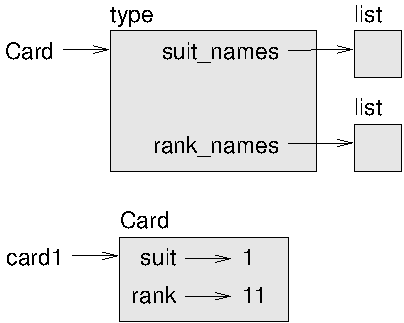
\includegraphics[scale=0.8]{figs/card1.pdf}}
\caption{Object diagram.}
\label{fig.card1}
\end{figure}

Figure~\ref{fig.card1} is a diagram of the {\tt Card} class object
and one Card instance.
\index{state diagram}
\index{diagram!state}
\index{object diagram}
\index{diagram!object}
{\tt Card} is a class object, so it has type {\tt type}.  {\tt
card1} has type {\tt Card}.  (To save space, I didn't draw the
contents of \verb"suit_names" and \verb"rank_names").


\section{Comparing cards}
\label{comparecard}
\index{operator!relational}
\index{relational operator}

For built-in types, there are relational operators
({\tt <}, {\tt >}, {\tt ==}, etc.)
that compare
values and determine when one is greater than, less than, or equal to
another.  For user-defined types, we can override the behavior of
the built-in operators by providing a method named
\verb"__cmp__".

\verb"__cmp__" takes two parameters, {\tt self} and {\tt other},
and returns a positive number if the first object is greater, a
negative number if the second object is greater, and 0 if they are
equal to each other.
\index{override}
\index{operator overloading}

The correct ordering for cards is not obvious.
For example, which
is better, the 3 of Clubs or the 2 of Diamonds?  One has a higher
rank, but the other has a higher suit.  In order to compare
cards, you have to decide whether rank or suit is more important.

The answer might depend on what game you are playing, but to keep
things simple, we'll make the arbitrary choice that suit is more
important, so all of the Spades outrank all of the Diamonds,
and so on.
\index{cmp method@\_\_cmp\_\_ method}
\index{method!\_\_cmp\_\_}

With that decided, we can write \verb"__cmp__":

\begin{verbatim}
# inside class Card:

    def __cmp__(self, other):
        # check the suits
        if self.suit > other.suit: return 1
        if self.suit < other.suit: return -1

        # suits are the same... check ranks
        if self.rank > other.rank: return 1
        if self.rank < other.rank: return -1

        # ranks are the same... it's a tie
        return 0
\end{verbatim}
%
You can write this more concisely using tuple comparison:
\index{tuple!comparison}
\index{comparison!tuple}

\begin{verbatim}
# inside class Card:

    def __cmp__(self, other):
        t1 = self.suit, self.rank
        t2 = other.suit, other.rank
        return cmp(t1, t2)
\end{verbatim}
%
The built-in function {\tt cmp} has the same interface as
the method \verb"__cmp__": it takes two values and returns
a positive number if the first is larger, a negative number
if the second is larger, and 0 if they are equal.
\index{cmp function}
\index{function!cmp}

In Python 3, {\tt cmp} no longer exists, and the \verb"__cmp__"
method is not supported.  Instead you should provide \verb"__lt__",
which returns {\tt True} if {\tt self} is less than {\tt other}.
You can implement \verb"__lt__" using tuples and the \verb"<"
operator.

\begin{exercise}

Write a \verb"__cmp__" method for Time objects.  Hint: you
can use tuple comparison, but you also might consider using
integer subtraction.

%    def __cmp__(self, other):
%        return time_to_int(self) - time_to_int(other)

%If {\tt self} is later than {\tt other}, the result is
%a positive number.  If {\tt other} is later, the result
%is negative.  And if {\tt self} and {\tt other} are equal
%(but not necessarily identical)
%the result is zero.

\end{exercise}


\section{Decks}
\index{list!of objects}
\index{deck, playing cards}

Now that we have Cards, the next step is to define Decks.  Since a
deck is made up of cards, it is natural for each Deck to contain a
list of cards as an attribute.
\index{init method}
\index{method!init}

The following is a class definition for {\tt Deck}.  The
init method creates the attribute {\tt cards} and generates
the standard set of fifty-two cards:
\index{composition}
\index{loop!nested}
\index{Deck class}
\index{class!Deck}

\begin{verbatim}
class Deck(object):

    def __init__(self):
        self.cards = []
        for suit in range(4):
            for rank in range(1, 14):
                card = Card(suit, rank)
                self.cards.append(card)
\end{verbatim}
%
The easiest way to populate the deck is with a nested loop.  The outer
loop enumerates the suits from 0 to 3.  The inner loop enumerates the
ranks from 1 to 13.  Each iteration
creates a new Card with the current suit and rank,
and appends it to {\tt self.cards}.
\index{append method}
\index{method!append}


\section{Printing the deck}
\label{printdeck}
\index{str method@\_\_str\_\_ method}
\index{method!\_\_str\_\_}

Here is a \verb"__str__" method for {\tt Deck}:

\begin{verbatim}
#inside class Deck:

    def __str__(self):
        res = []
        for card in self.cards:
            res.append(str(card))
        return '\n'.join(res)
\end{verbatim}
%
This method demonstrates an efficient way to accumulate a large
string: building a list of strings and then using {\tt join}.
The built-in function {\tt str} invokes the \verb"__str__"
method on each card and returns the string representation.
\index{accumulator!string}
\index{string!accumulator}
\index{join method}
\index{method!join}
\index{newline}

Since we invoke {\tt join} on a newline character, the cards
are separated by newlines.  Here's what the result looks like:

\begin{verbatim}
>>> deck = Deck()
>>> print deck
Ace of Clubs
2 of Clubs
3 of Clubs
...
10 of Spades
Jack of Spades
Queen of Spades
King of Spades
\end{verbatim}
%
Even though the result appears on 52 lines, it is
one long string that contains newlines.


\section{Add, remove, shuffle and sort}

To deal cards, we would like a method that
removes a card from the deck and returns it.
The list method {\tt pop} provides a convenient way to do that:
\index{pop method}
\index{method!pop}

\begin{verbatim}
#inside class Deck:

    def pop_card(self):
        return self.cards.pop()
\end{verbatim}
%
Since {\tt pop} removes the {\em last} card in the list, we are
dealing from the bottom of the deck.  In real life ``bottom dealing'' is
frowned upon,
but in this context it's ok.
\index{append method}
\index{method!append}

To add a card, we can use the list method {\tt append}:

\begin{verbatim}
#inside class Deck:

    def add_card(self, card):
        self.cards.append(card)
\end{verbatim}
%
A method like this that uses another function without doing
much real work is sometimes called a {\bf veneer}.  The metaphor
comes from woodworking, where it is common to glue a thin
layer of good quality wood to the surface of a cheaper piece of
wood.
\index{veneer}

In this case we are defining a ``thin'' method that expresses
a list operation in terms that are appropriate for decks.

As another example, we can write a Deck method named {\tt shuffle}
using the function {\tt shuffle} from the {\tt random} module:
\index{random module}
\index{module!random}
\index{shuffle function}
\index{function!shuffle}

\begin{verbatim}
# inside class Deck:

    def shuffle(self):
        random.shuffle(self.cards)
\end{verbatim}
%
Don't forget to import {\tt random}.

\begin{exercise}
\index{sort method}
\index{method!sort}

Write a Deck method named {\tt sort} that uses the list method
{\tt sort} to sort the cards in a {\tt Deck}.  {\tt sort} uses
the \verb"__cmp__" method we defined to determine sort order.
\end{exercise}



\section{Inheritance}
\index{inheritance}
\index{object-oriented programming}

The language feature most often associated with object-oriented
programming is {\bf inheritance}.  Inheritance is the ability to
define a new class that is a modified version of an existing
class.
\index{parent class}
\index{child class}
\index{class!child}
\index{subclass}
\index{superclass}

It is called ``inheritance'' because the new class inherits the
methods of the existing class.  Extending this metaphor, the existing
class is called the {\bf parent} and the new class is
called the {\bf child}.

As an example, let's say we want a class to represent a ``hand,''
that is, the set of cards held by one player.  A hand is similar to a
deck: both are made up of a set of cards, and both require operations
like adding and removing cards.

A hand is also different from a deck; there are operations we want for
hands that don't make sense for a deck.  For example, in poker we
might compare two hands to see which one wins.  In bridge, we might
compute a score for a hand in order to make a bid.

This relationship between classes---similar, but different---lends
itself to inheritance.

The definition of a child class is like other class definitions,
but the name of the parent class appears in parentheses:
\index{parentheses!parent class in}
\index{parent class}
\index{class!parent}
\index{Hand class}
\index{class!Hand}

\begin{verbatim}
class Hand(Deck):
    """Represents a hand of playing cards."""
\end{verbatim}
%
This definition indicates that {\tt Hand} inherits from {\tt Deck};
that means we can use methods like \verb"pop_card" and \verb"add_card"
for Hands as well as Decks.

{\tt Hand} also inherits \verb"__init__" from {\tt Deck}, but
it doesn't really do what we want: instead of populating the hand
with 52 new cards, the init method for Hands should initialize
{\tt cards} with an empty list.
\index{override}
\index{init method}
\index{method!init}

If we provide an init method in the {\tt Hand} class, it overrides the
one in the {\tt Deck} class:

\begin{verbatim}
# inside class Hand:

    def __init__(self, label=''):
        self.cards = []
        self.label = label
\end{verbatim}
%
So when you create a Hand, Python invokes this init method:

\begin{verbatim}
>>> hand = Hand('new hand')
>>> print hand.cards
[]
>>> print hand.label
new hand
\end{verbatim}
%
But the other methods are inherited from {\tt Deck}, so we can use
\verb"pop_card" and \verb"add_card" to deal a card:

\begin{verbatim}
>>> deck = Deck()
>>> card = deck.pop_card()
>>> hand.add_card(card)
>>> print hand
King of Spades
\end{verbatim}
%
A natural next step is to encapsulate this code in a method
called \verb"move_cards":
\index{encapsulation}

\begin{verbatim}
#inside class Deck:

    def move_cards(self, hand, num):
        for i in range(num):
            hand.add_card(self.pop_card())
\end{verbatim}
%
\verb"move_cards" takes two arguments, a Hand object and the number of
cards to deal.  It modifies both {\tt self} and {\tt hand}, and
returns {\tt None}.

In some games, cards are moved from one hand to another,
or from a hand back to the deck.  You can use \verb"move_cards"
for any of these operations: {\tt self} can be either a Deck
or a Hand, and {\tt hand}, despite the name, can also be a {\tt Deck}.

\begin{exercise}

Write a Deck method called \verb"deal_hands" that takes two
parameters, the number of hands and the number of cards per
hand, and that creates new Hand objects, deals the appropriate
number of cards per hand, and returns a list of Hand objects.

\end{exercise}

Inheritance is a useful feature.  Some programs that would be
repetitive without inheritance can be written more elegantly
with it.  Inheritance can facilitate code reuse, since you can
customize the behavior of parent classes without having to modify
them.  In some cases, the inheritance structure reflects the natural
structure of the problem, which makes the program easier to
understand.

On the other hand, inheritance can make programs difficult to read.
When a method is invoked, it is sometimes not clear where to find its
definition.  The relevant code may be scattered among several modules.
Also, many of the things that can be done using inheritance can be
done as well or better without it.


\section{Class diagrams}
\label{class.diagram}

So far we have seen stack diagrams, which show the state of
a program, and object diagrams, which show the attributes
of an object and their values.  These diagrams represent a snapshot
in the execution of a program, so they change as the program
runs.

They are also highly detailed; for some purposes, too
detailed.  A class diagram is a more abstract representation
of the structure of a program.  Instead of showing individual
objects, it shows classes and the relationships between them.

There are several kinds of relationship between classes:

\begin{itemize}

\item Objects in one class might contain references to objects
in another class.  For example, each Rectangle contains a reference
to a Point, and each Deck contains references to many Cards.
This kind of relationship is called {\bf HAS-A}, as in, ``a Rectangle
has a Point.''

\item One class might inherit from another.  This relationship
is called {\bf IS-A}, as in, ``a Hand is a kind of a Deck.''

\item One class might depend on another in the sense that changes
in one class would require changes in the other.

\end{itemize}
\index{IS-A relationship}
\index{HAS-A relationship}
\index{class diagram}
\index{diagram!class}

A {\bf class diagram} is a graphical representation of these
relationships.  For example, Figure~\ref{fig.class1} shows the
relationships between {\tt Card}, {\tt Deck} and {\tt Hand}.

\begin{figure}
\centerline
{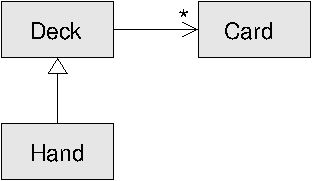
\includegraphics[scale=0.8]{figs/class1.pdf}}
\caption{Class diagram.}
\label{fig.class1}
\end{figure}


The arrow with a hollow triangle head represents an IS-A
relationship; in this case it indicates that Hand inherits
from Deck.

The standard arrow head represents a HAS-A
relationship; in this case a Deck has references to Card
objects.
\index{multiplicity (in class diagram)}

The star ({\tt *}) near the arrow head is a
{\bf multiplicity}; it indicates how many Cards a Deck has.
A multiplicity can be a simple number, like {\tt 52}, a range,
like {\tt 5..7} or a star, which indicates that a Deck can
have any number of Cards.

A more detailed diagram might show that a Deck actually
contains a {\em list} of Cards, but built-in types
like list and dict are usually not included in class diagrams.

\begin{exercise}

Read {\tt TurtleWorld.py}, {\tt World.py} and {\tt Gui.py}
and draw a class diagram that shows the relationships among
the classes defined there.

\end{exercise}


\section{Debugging}
\index{debugging}

Inheritance can make debugging a challenge because when you
invoke a method on an object, you might not know which method
will be invoked.
\index{polymorphism}

Suppose you are writing a function that works with Hand objects.
You would like it to work with all kinds of Hands, like
PokerHands, BridgeHands, etc.  If you invoke a method like
{\tt shuffle}, you might get the one defined in {\tt Deck},
but if any of the subclasses override this method, you'll
get that version instead.
\index{flow of execution}

Any time you are unsure about the flow of execution through your
program, the simplest solution is to add print statements at the
beginning of the relevant methods.  If {\tt Deck.shuffle} prints a
message that says something like {\tt Running Deck.shuffle}, then as
the program runs it traces the flow of execution.

As an alternative, you could use this function, which takes an
object and a method name (as a string) and returns the class that
provides the definition of the method:

\begin{verbatim}
def find_defining_class(obj, meth_name):
    for ty in type(obj).mro():
        if meth_name in ty.__dict__:
            return ty
\end{verbatim}
%
Here's an example:

\begin{verbatim}
>>> hand = Hand()
>>> print find_defining_class(hand, 'shuffle')
<class 'Card.Deck'>
\end{verbatim}
%
So the {\tt shuffle} method for this Hand is the one in {\tt Deck}.
\index{mro method}
\index{method!mro}
\index{method resolution order}

\verb"find_defining_class" uses the {\tt mro} method to get the list
of class objects (types) that will be searched for methods.  ``MRO''
stands for ``method resolution order.''
\index{override}
\index{interface}
\index{precondition}
\index{postcondition}

Here's a program design suggestion: whenever you override a method,
the interface of the new method should be the same as the old.  It
should take the same parameters, return the same type, and obey the
same preconditions and postconditions.  If you obey this rule, you
will find that any function designed to work with an instance of a
superclass, like a Deck, will also work with instances of subclasses
like a Hand or PokerHand.

If you violate this rule, your code will collapse like (sorry)
a house of cards.


\section{Data encapsulation}

Chapter~\ref{time} demonstrates a development plan we might call
``object-oriented design.''  We identified objects we needed---{\tt
  Time}, {\tt Point} and {\tt Rectangle}---and defined classes to
represent them.  In each case there is an obvious correspondence
between the object and some entity in the real world (or at least a
mathematical world).
\index{development plan}

But sometimes it is less obvious what objects you need
and how they should interact.  In that case you need a different
development plan.  In the same way that we discovered function
interfaces by encapsulation and generalization, we can discover
class interfaces by {\bf data encapsulation}.
\index{data encapsulation}
\index{encapsulation!data}

Markov analysis, from Section~\ref{markov}, provides a good example.
If you download my code from \url{http://thinkpython.com/code/markov.py},
you'll see that it uses two global variables---\verb"suffix_map" and
\verb"prefix"---that are read and written from several functions.

\begin{verbatim}
suffix_map = {}
prefix = ()
\end{verbatim}

Because these variables are global
we can only run one analysis
at a time.  If we read two texts, their prefixes and suffixes would
be added to the same data structures (which makes for some interesting
generated text).

To run multiple analyses, and keep them separate, we can encapsulate
the state of each analysis in an object.
Here's what that looks like:

\begin{verbatim}
class Markov(object):

    def __init__(self):
        self.suffix_map = {}
        self.prefix = ()
\end{verbatim}

Next, we transform the functions into methods.  For example,
here's \verb"process_word":

\begin{verbatim}
    def process_word(self, word, order=2):
        if len(self.prefix) < order:
            self.prefix += (word,)
            return

        try:
            self.suffix_map[self.prefix].append(word)
        except KeyError:
            # if there is no entry for this prefix, make one
            self.suffix_map[self.prefix] = [word]

        self.prefix = shift(self.prefix, word)
\end{verbatim}

Transforming a program like this---changing the design without
changing the function---is another example of refactoring
(see Section~\ref{refactoring}).
\index{refactoring}

This example suggests a development plan for designing objects and
methods:

\begin{enumerate}

\item Start by writing functions that read and write global
variables (when necessary).

\item Once you get the program working, look for associations
between global variables and the functions that use them.

\item Encapsulate related variables as attributes of an object.

\item Transform the associated functions into methods of the new
class.

\end{enumerate}


\begin{exercise}

Download my code from Section~\ref{markov}
(\url{http://thinkpython.com/code/markov.py}), and follow the steps described
above to encapsulate the global variables as attributes of a new class
called {\tt Markov}.  Solution: \url{http://thinkpython.com/code/Markov.py}
(note the capital M).

\end{exercise}




\section{Glossary}

\begin{description}

\item[encode:]  To represent one set of values using another
set of values by constructing a mapping between them.
\index{encode}

\item[class attribute:] An attribute associated with a class
object.  Class attributes are defined inside
a class definition but outside any method.
\index{class attribute}
\index{attribute!class}

\item[instance attribute:] An attribute associated with an
instance of a class.
\index{instance attribute}
\index{attribute!instance}

\item[veneer:] A method or function that provides a different
interface to another function without doing much computation.
\index{veneer}

\item[inheritance:] The ability to define a new class that is a
modified version of a previously defined class.
\index{inheritance}

\item[parent class:] The class from which a child class inherits.
\index{parent class}

\item[child class:] A new class created by inheriting from an
existing class; also called a ``subclass.''
\index{child class}
\index{class!child}

\item[IS-A relationship:] The relationship between a child class
and its parent class.
\index{IS-A relationship}

\item[HAS-A relationship:] The relationship between two classes
where instances of one class contain references to instances of
the other.
\index{HAS-A relationship}

\item[class diagram:] A diagram that shows the classes in a program
and the relationships between them.
\index{class diagram}
\index{diagram!class}

\item[multiplicity:] A notation in a class diagram that shows, for
a HAS-A relationship, how many references there are to instances
of another class.
\index{multiplicity (in class diagram)}

\end{description}


\section{Exercises}

\begin{exercise}
\label{poker}

The following are the possible hands in poker, in increasing order
of value (and decreasing order of probability):
\index{poker}

\begin{description}

\item[pair:] two cards with the same rank
\vspace{-0.05in}

\item[two pair:] two pairs of cards with the same rank
\vspace{-0.05in}

\item[three of a kind:] three cards with the same rank
\vspace{-0.05in}

\item[straight:] five cards with ranks in sequence (aces can
be high or low, so {\tt Ace-2-3-4-5} is a straight and so is {\tt
10-Jack-Queen-King-Ace}, but {\tt Queen-King-Ace-2-3} is not.)
\vspace{-0.05in}

\item[flush:] five cards with the same suit
\vspace{-0.05in}

\item[full house:] three cards with one rank, two cards with another
\vspace{-0.05in}

\item[four of a kind:] four cards with the same rank
\vspace{-0.05in}

\item[straight flush:] five cards in sequence (as defined above) and
with the same suit
\vspace{-0.05in}

\end{description}
%
The goal of these exercises is to estimate
the probability of drawing these various hands.

\begin{enumerate}

\item Download the following files from \url{http://thinkpython.com/code}:

\begin{description}

\item[{\tt Card.py}]: A complete version of the {\tt Card},
{\tt Deck} and {\tt Hand} classes in this chapter.

\item[{\tt PokerHand.py}]: An incomplete implementation of a class
that represents a poker hand, and some code that tests it.

\end{description}
%
\item If you run {\tt PokerHand.py}, it deals seven 7-card poker hands
and checks to see if any of them contains a flush.  Read this
code carefully before you go on.

\item Add methods to {\tt PokerHand.py} named \verb"has_pair",
\verb"has_twopair", etc. that return True or False according to
whether or not the hand meets the relevant criteria.  Your code should
work correctly for ``hands'' that contain any number of cards
(although 5 and 7 are the most common sizes).

\item Write a method named {\tt classify} that figures out
the highest-value classification for a hand and sets the
{\tt label} attribute accordingly.  For example, a 7-card hand
might contain a flush and a pair; it should be labeled ``flush''.

\item When you are convinced that your classification methods are
working, the next step is to estimate the probabilities of the various
hands.  Write a function in {\tt PokerHand.py} that shuffles a deck of
cards, divides it into hands, classifies the hands, and counts the
number of times various classifications appear.

\item Print a table of the classifications and their probabilities.
Run your program with larger and larger numbers of hands until the
output values converge to a reasonable degree of accuracy.  Compare
your results to the values at \url{http://en.wikipedia.org/wiki/Hand_rankings}.

\end{enumerate}

Solution: \url{http://thinkpython.com/code/PokerHandSoln.py}.
\end{exercise}


\begin{exercise}
\index{Swampy}
\index{TurtleWorld}

This exercise uses TurtleWorld from Chapter~\ref{turtlechap}.
You will write code that makes Turtles play tag.  If you
are not familiar with the rules of tag, see
\url{http://en.wikipedia.org/wiki/Tag_(game)}.

\begin{enumerate}

\item Download \url{http://thinkpython.com/code/Wobbler.py} and run it.  You
should see a TurtleWorld with three Turtles.  If you press the
{\sf Run} button, the Turtles wander at random.

\item Read the code and make sure you understand how it works.
The {\tt Wobbler} class inherits from {\tt Turtle}, which means
that the {\tt Turtle} methods {\tt lt}, {\tt rt}, {\tt fd}
and {\tt bk} work on Wobblers.

The {\tt step} method gets invoked by TurtleWorld.  It invokes
{\tt steer}, which turns the Turtle in the desired direction,
{\tt wobble}, which makes a random turn in proportion to the Turtle's
clumsiness, and {\tt move}, which moves forward a few pixels,
depending on the Turtle's speed.
\index{Tagger}

\item Create a file named {\tt Tagger.py}.  Import everything from
  {\tt Wobbler}, then define a class named {\tt Tagger} that inherits
  from {\tt Wobbler}.  Call \verb"make_world" passing the {\tt
    Tagger} class object as an argument.

\item Add a {\tt steer} method to {\tt Tagger} to override the one in
  {\tt Wobbler}.  As a starting place, write a version that always
  points the Turtle toward the origin.  Hint: use the math function
  {\tt atan2} and the Turtle attributes {\tt x}, {\tt y} and
  {\tt heading}.

\item Modify {\tt steer} so that the Turtles stay in bounds.
  For debugging, you might want to use the {\sf Step} button,
  which invokes {\tt step} once on each Turtle.

\item Modify {\tt steer} so that each Turtle points toward its nearest
  neighbor.  Hint: Turtles have an attribute, {\tt world}, that is a
  reference to the TurtleWorld they live in, and the TurtleWorld has
  an attribute, {\tt animals}, that is a list of all Turtles in the
  world.

\item Modify {\tt steer} so the Turtles play tag.  You can add methods
  to {\tt Tagger} and you can override {\tt steer} and
  \verb"__init__", but you may not modify or override {\tt step}, {\tt
    wobble} or {\tt move}.  Also, {\tt steer} is allowed to change the
  heading of the Turtle but not the position.

Adjust the rules and your {\tt steer} method for good quality play;
for example, it should be possible for the slow Turtle to tag the
faster Turtles eventually.

\end{enumerate}

Solution: \url{http://thinkpython.com/code/Tagger.py}.
\end{exercise}
